\documentclass{article}

%--------------------------------------------------------------
% Document & Font Setup
%--------------------------------------------------------------
\usepackage[a4paper, margin=1in]{geometry}
\usepackage{setspace}
\usepackage{parskip}
%--------------------------------------------------------------
% Common Packages
%--------------------------------------------------------------
\usepackage{graphicx}
\usepackage{subcaption}
\usepackage{caption}
% Subfigure captions
\DeclareCaptionLabelFormat{custom}{\figurename~\thefigure~(#2)}
\captionsetup[subfigure]{labelformat=custom}

\usepackage{enumitem}
\usepackage{float}
\usepackage{placeins}
\usepackage[dvipsnames,x11names,svgnames]{xcolor}
\usepackage{url}

%--------------------------------------------------------------
% Math & Science Packages
%--------------------------------------------------------------
\usepackage{amsmath,amssymb,amsfonts,amsthm}
\usepackage{mathtools}
\usepackage{bbm}
\usepackage{siunitx}
\DeclareSIUnit{\rpm}{RPM}
\DeclareSIUnit{\au}{AU}

%--------------------------------------------------------------
% Hyperlinks
%--------------------------------------------------------------
\usepackage{hyperref}
\hypersetup{
    hidelinks,
    colorlinks=true,
    linkcolor=blue,
    urlcolor=red
}

%--------------------------------------------------------------
% Headers & Footers
%--------------------------------------------------------------
\usepackage{fancyhdr, lastpage}

\fancypagestyle{mainmatter}{
    \fancyhf{}
    \lhead{2025}
    \rhead{EPSRC}
    \cfoot{Page \thepage\ of \pageref{LastPage}}
    \renewcommand{\headrulewidth}{0.4pt}
    \renewcommand{\footrulewidth}{0.4pt}
}

%--------------------------------------------------------------
% Todo
%--------------------------------------------------------------
\usepackage{todonotes}

%--------------------------------------------------------------
% Plots & Graphics
%--------------------------------------------------------------
\usepackage{pgfplots}
\pgfplotsset{compat=1.18}
\usepackage{tikz}

% TikZ
\usetikzlibrary{
    shapes.geometric,
    shapes.misc,
    arrows.meta,
    positioning,
    matrix,
    calc,
    fit,
    fadings,
    patterns,
    plotmarks,
    decorations.pathmorphing
}
\tikzset{font={\fontsize{10pt}{12}\selectfont}}
\tikzset{
    startstop/.style = {rectangle, rounded corners, ...},
    IO/.style        = {ellipse, ...},
    arrow/.style     = {thick,->,>={Stealth}},
    block/.style     = {rectangle, draw, ...},
    sum/.style       = {draw, circle, ...},
    bag/.style       = {align=left}
}

% Custom colors
\definecolor{sandybrown}{rgb}{0.96, 0.64, 0.38}

%--------------------------------------------------------------
% Custom Commands, Environments, & Numbering
%--------------------------------------------------------------
\numberwithin{equation}{section}
\numberwithin{figure}{section}
\numberwithin{table}{section}
\numberwithin{algorithm}{section}

\newtheorem{property}{Property}[section]
\newtheorem{theorem}{Theorem}[section]
\newtheorem{corollary}{Corollary}[section]
\newtheorem{definition}{Definition}[section]
\newtheorem{assumption}{Assumption}[section]

\DeclareMathOperator*{\argmax}{arg\,max}
\DeclareMathOperator*{\argmin}{arg\,min}
\newcommand{\defeq}{\vcentcolon=}
\newcommand{\traj}{\{x(k)\}_{k=0,\dots,T}}
\newcommand{\dgap}{d}
\newcommand\given[1][]{\:#1\vert\:}

\let\oldemptyset\emptyset
\let\emptyset\varnothing

\newcommand\blfootnote[1]{%
  \begingroup
  \renewcommand\thefootnote{}\footnote{#1}%
  \addtocounter{footnote}{-1}%
  \endgroup
}
\usepackage[backend=bibtex, sorting=none]{biblatex}
\addbibresource{bibliography.bib}


\title{Project 1: Empirical Observation of the Starlink-3988 Satellite}
\author{Claudio Vestini}


\begin{document}

\maketitle

\section{Introduction \& Satellite Selection}

Since the first successful deployment of a human-made object into Earth's orbit with \textit{Sputnik 1} in 1957, over 15,000 satellites have been placed in orbit around our planet~\cite{lookup-lepoint2025}. Of these, more than 13,000 remain operational today, and this unprecedented active percentage is continuously growing. The vast majority are of American origin (roughly \SI{74}{\percent}), and most belong to SpaceX's Starlink constellation, which alone accounts for approximately \SI{86}{\percent} of all U.S. satellites and \SI{64}{\percent} of the world's total active population. Engineered to provide high-speed, low-latency internet connectivity to underserved rural areas of the world for a moderate service price, Starlink has been rapidly expanding its constellation, with thousands of new satellites being launched every year through proprietary SpaceX vehicles.

\begin{figure}[h!]
    \centering
    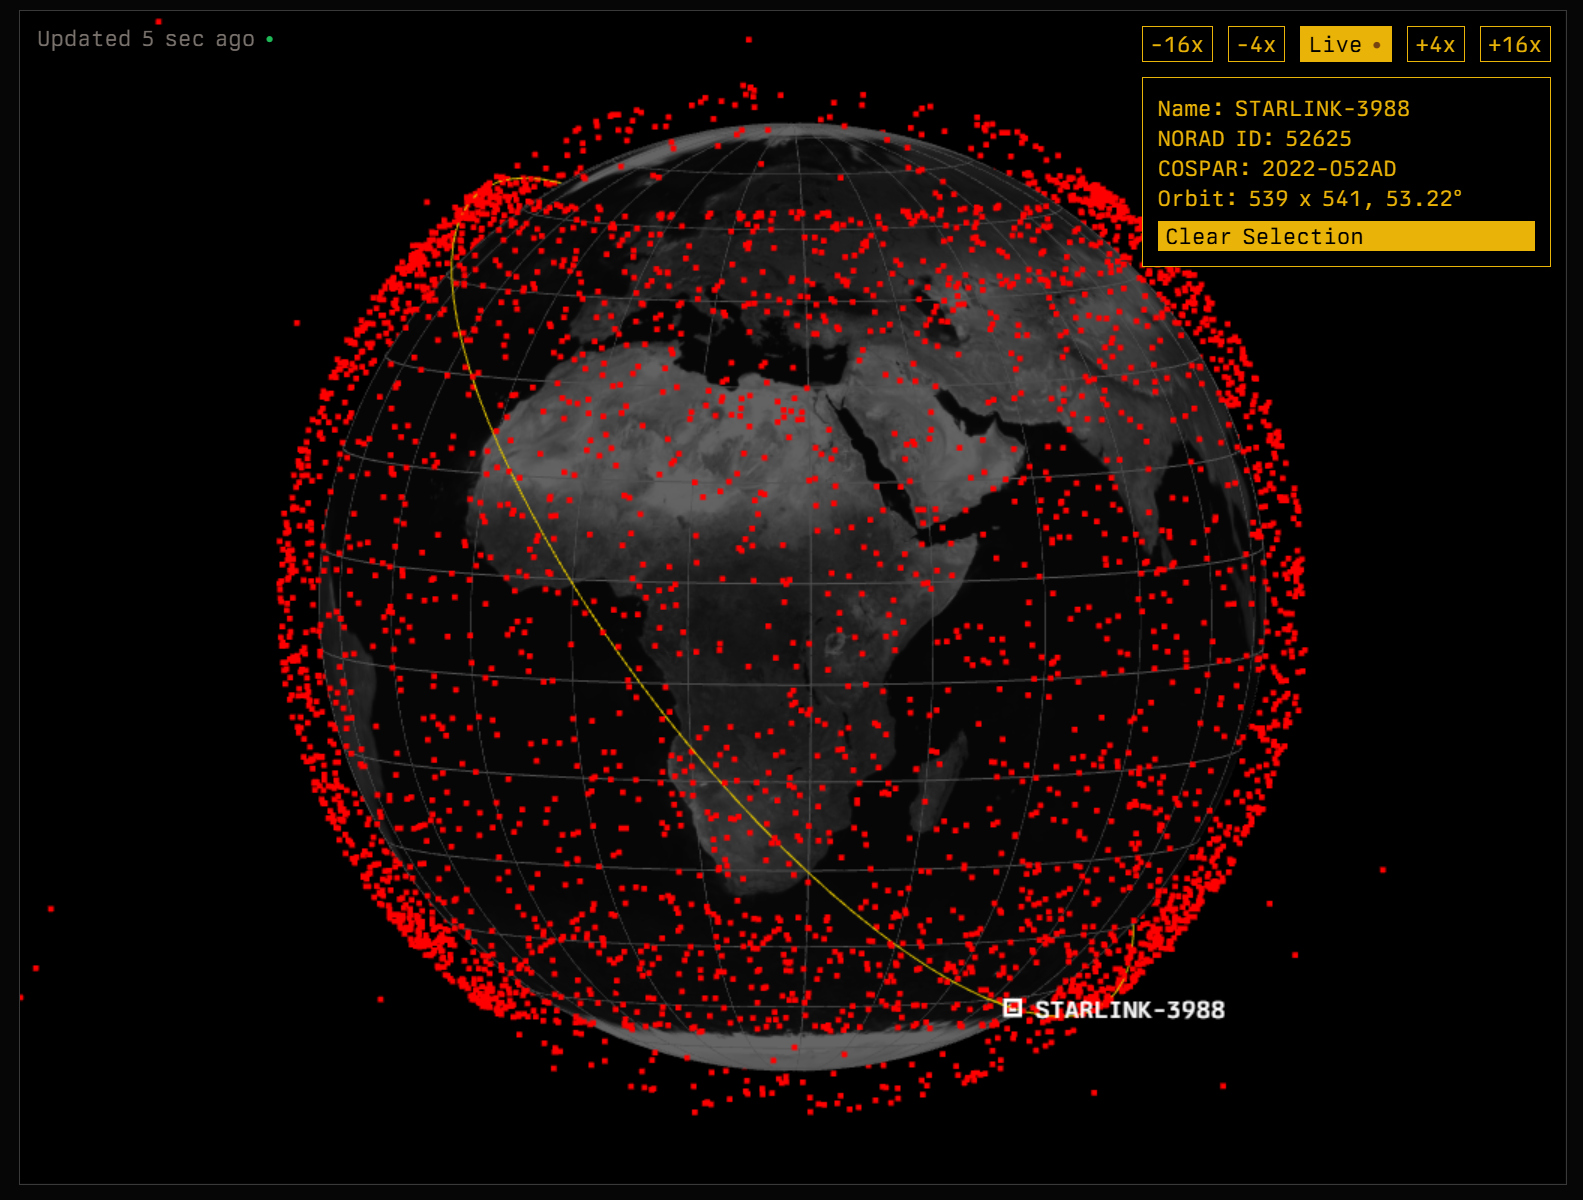
\includegraphics[width=\textwidth]{LaTeX/Figures/Starlink Constellation.png}
    \caption{Starlink constellation as of October 19th 2025, 16:59:33. Each red square represents an active satellite. Highlighted in yellow is the orbital track of selected satellite \textit{Starlink-3988}, with relevant orbital information displayed. The image is a screenshot from the Starlink Map website~\cite{starlinkmap.org}.}
    \label{fig:constellation}
\end{figure}

These satellites have already been used for several key applications, including enabling WiFi connectivity in commercial airlines and cruises, providing life-critical broadband in hurricane-ravaged coastal towns and earthquake-shaken regions, and facilitating allied command and control operations in the Russo-Ukrainian War. The constellation includes nearly 9,700 satellites (as of the writing of this report), and is visualised in Figure~\ref{fig:constellation}. Each unit is equipped with four beamforming, phased array antennas, each of which electronically steers the \SI{11.7}{\giga\hertz} collimated downlink signals in real time to a \SI{24}{\kilo\metre}-diameter ground coverage cell that can serve up to 8,000 simultaneous customers. Furthermore, the satellites communicate with one another via five on-board optical lasers at vacuum light-speed, enabling lower effective latencies between far-away cities compared to underwater cables. This is particularly relevant for applications in stock market trading, where saving a few milliseconds in latency can have a huge impact on the decision-making reactions to market fluctuations. To add to the list of groundbreaking engineering innovations that SpaceX developed for Starlink satellites, the orbital insertion procedure is entirely novel: the satellites are deployed in clusters of up to 23 units\footnote{For the larger v2 model, down from up to 60 units of the smaller v1/v1.5 model} at an altitude of roughly \SI{280}{\kilo\metre}, as shown in Figure~\ref{fig:starlink_cluster}; their orbits are then slowly raised to around \SI{550}{\kilo\metre} in two stages using Kripton gas ion thrusters\footnote{This is a more cost-efficient alternative to the customary option, Xenon gas}. This unusual manoeuvre leaves the satellites bunched up in characteristic lines before successful insertion, which can be observed from the surface of the Earth as shown in Figure~\ref{fig:starlink_line}.

\begin{figure}[h!]
    \centering

    % First subfigure (left image)
    \begin{subfigure}[b]{0.49\textwidth}
        \centering
        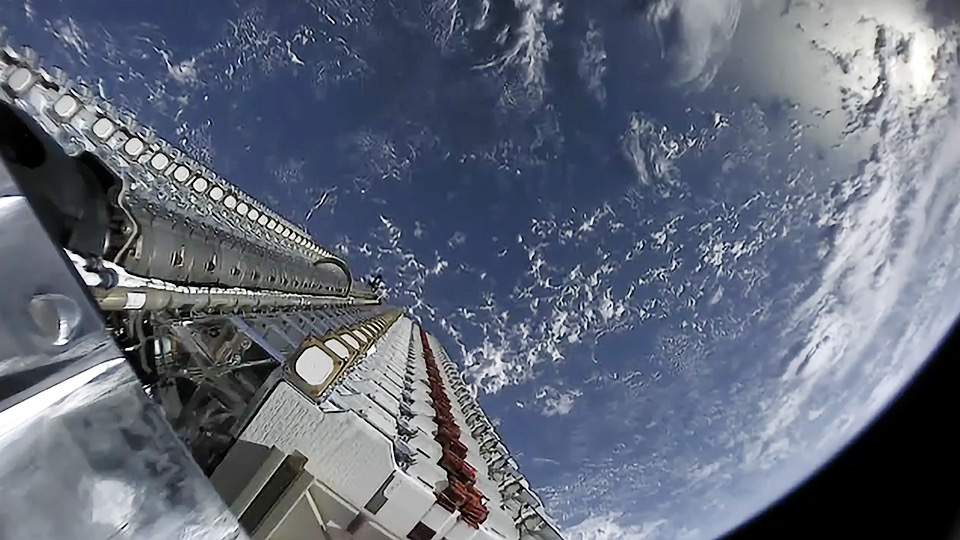
\includegraphics[width=\textwidth]{LaTeX/Figures/Starlink_cluster.jpg}
        \caption{A cluster of Starlink satellites. From~\cite{wikimedia_starlink_mission_2020}.}
        \label{fig:starlink_cluster}
    \end{subfigure}\hfill % No blank line between subfigures
    % Second subfigure (right image)
    \begin{subfigure}[b]{0.49\textwidth}
        \centering
        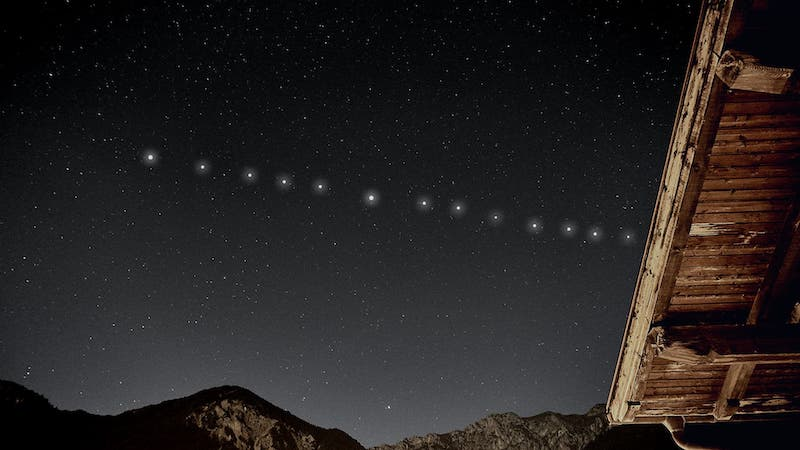
\includegraphics[width=\textwidth]{LaTeX/Figures/SPACEX-STARLINK-SATELLITES-CONSTELLATION.jpeg}
        \caption{A line of Starlink satellites. From~\cite{earthsky_starlink_2021}.}
        \label{fig:starlink_line}
    \end{subfigure}
    
\end{figure}

This project aims to investigate the orbit of an active, Earth-orbiting Starlink satellite through empirical observation and data collection. The satellite chosen is the \textit{Starlink-3988} unit, a v1.5 model as shown in Figure~\ref{fig:satellite_render}: although there aren't any attributes that distinguish it from others in the Starlink constellation, it was selected due to its favourable visibility and consistent orbital passes over Princeton, New Jersey, during the observation window (October 19–22, 2025). Furthermore, the satellite’s low-Earth orbit (LEO) characteristics, including a near-circular path, moderate inclination, and short orbital period, make it ideal for this project's requirements. A detail of the satellite's antennas is shown in Figure~\ref{fig:satellite_antennas}, and relevant attributes are reported in Table~\ref{tab:starlink3988_params}.

\begin{figure}[h!]
    \centering
    
    \begin{subfigure}[b]{0.49\textwidth}
        \centering
        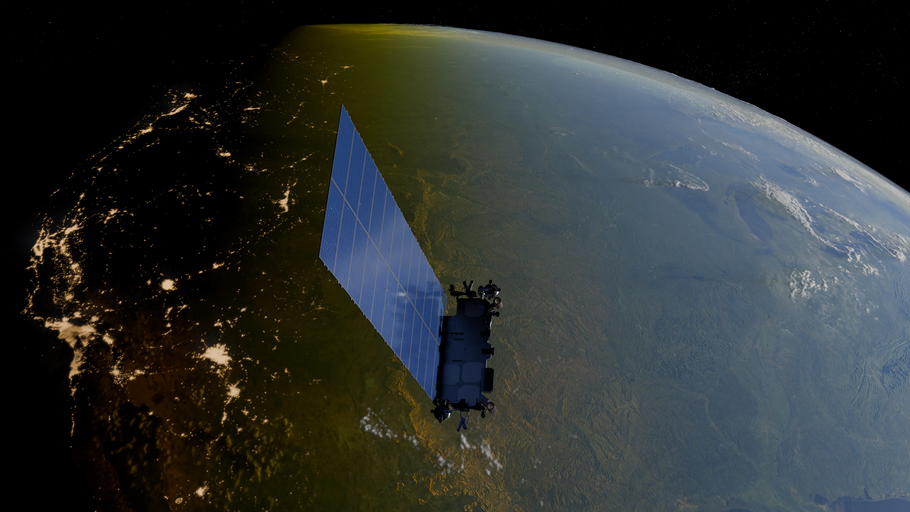
\includegraphics[width=\textwidth]{LaTeX/Figures/satellite_render.png}
        \caption{3D render of a Starlink v1.5 satellite~\cite{wikimedia_starlink_01_2025}.}
        \label{fig:satellite_render}
    \end{subfigure}\hfill
    \begin{subfigure}[b]{0.49\textwidth}
        \centering
        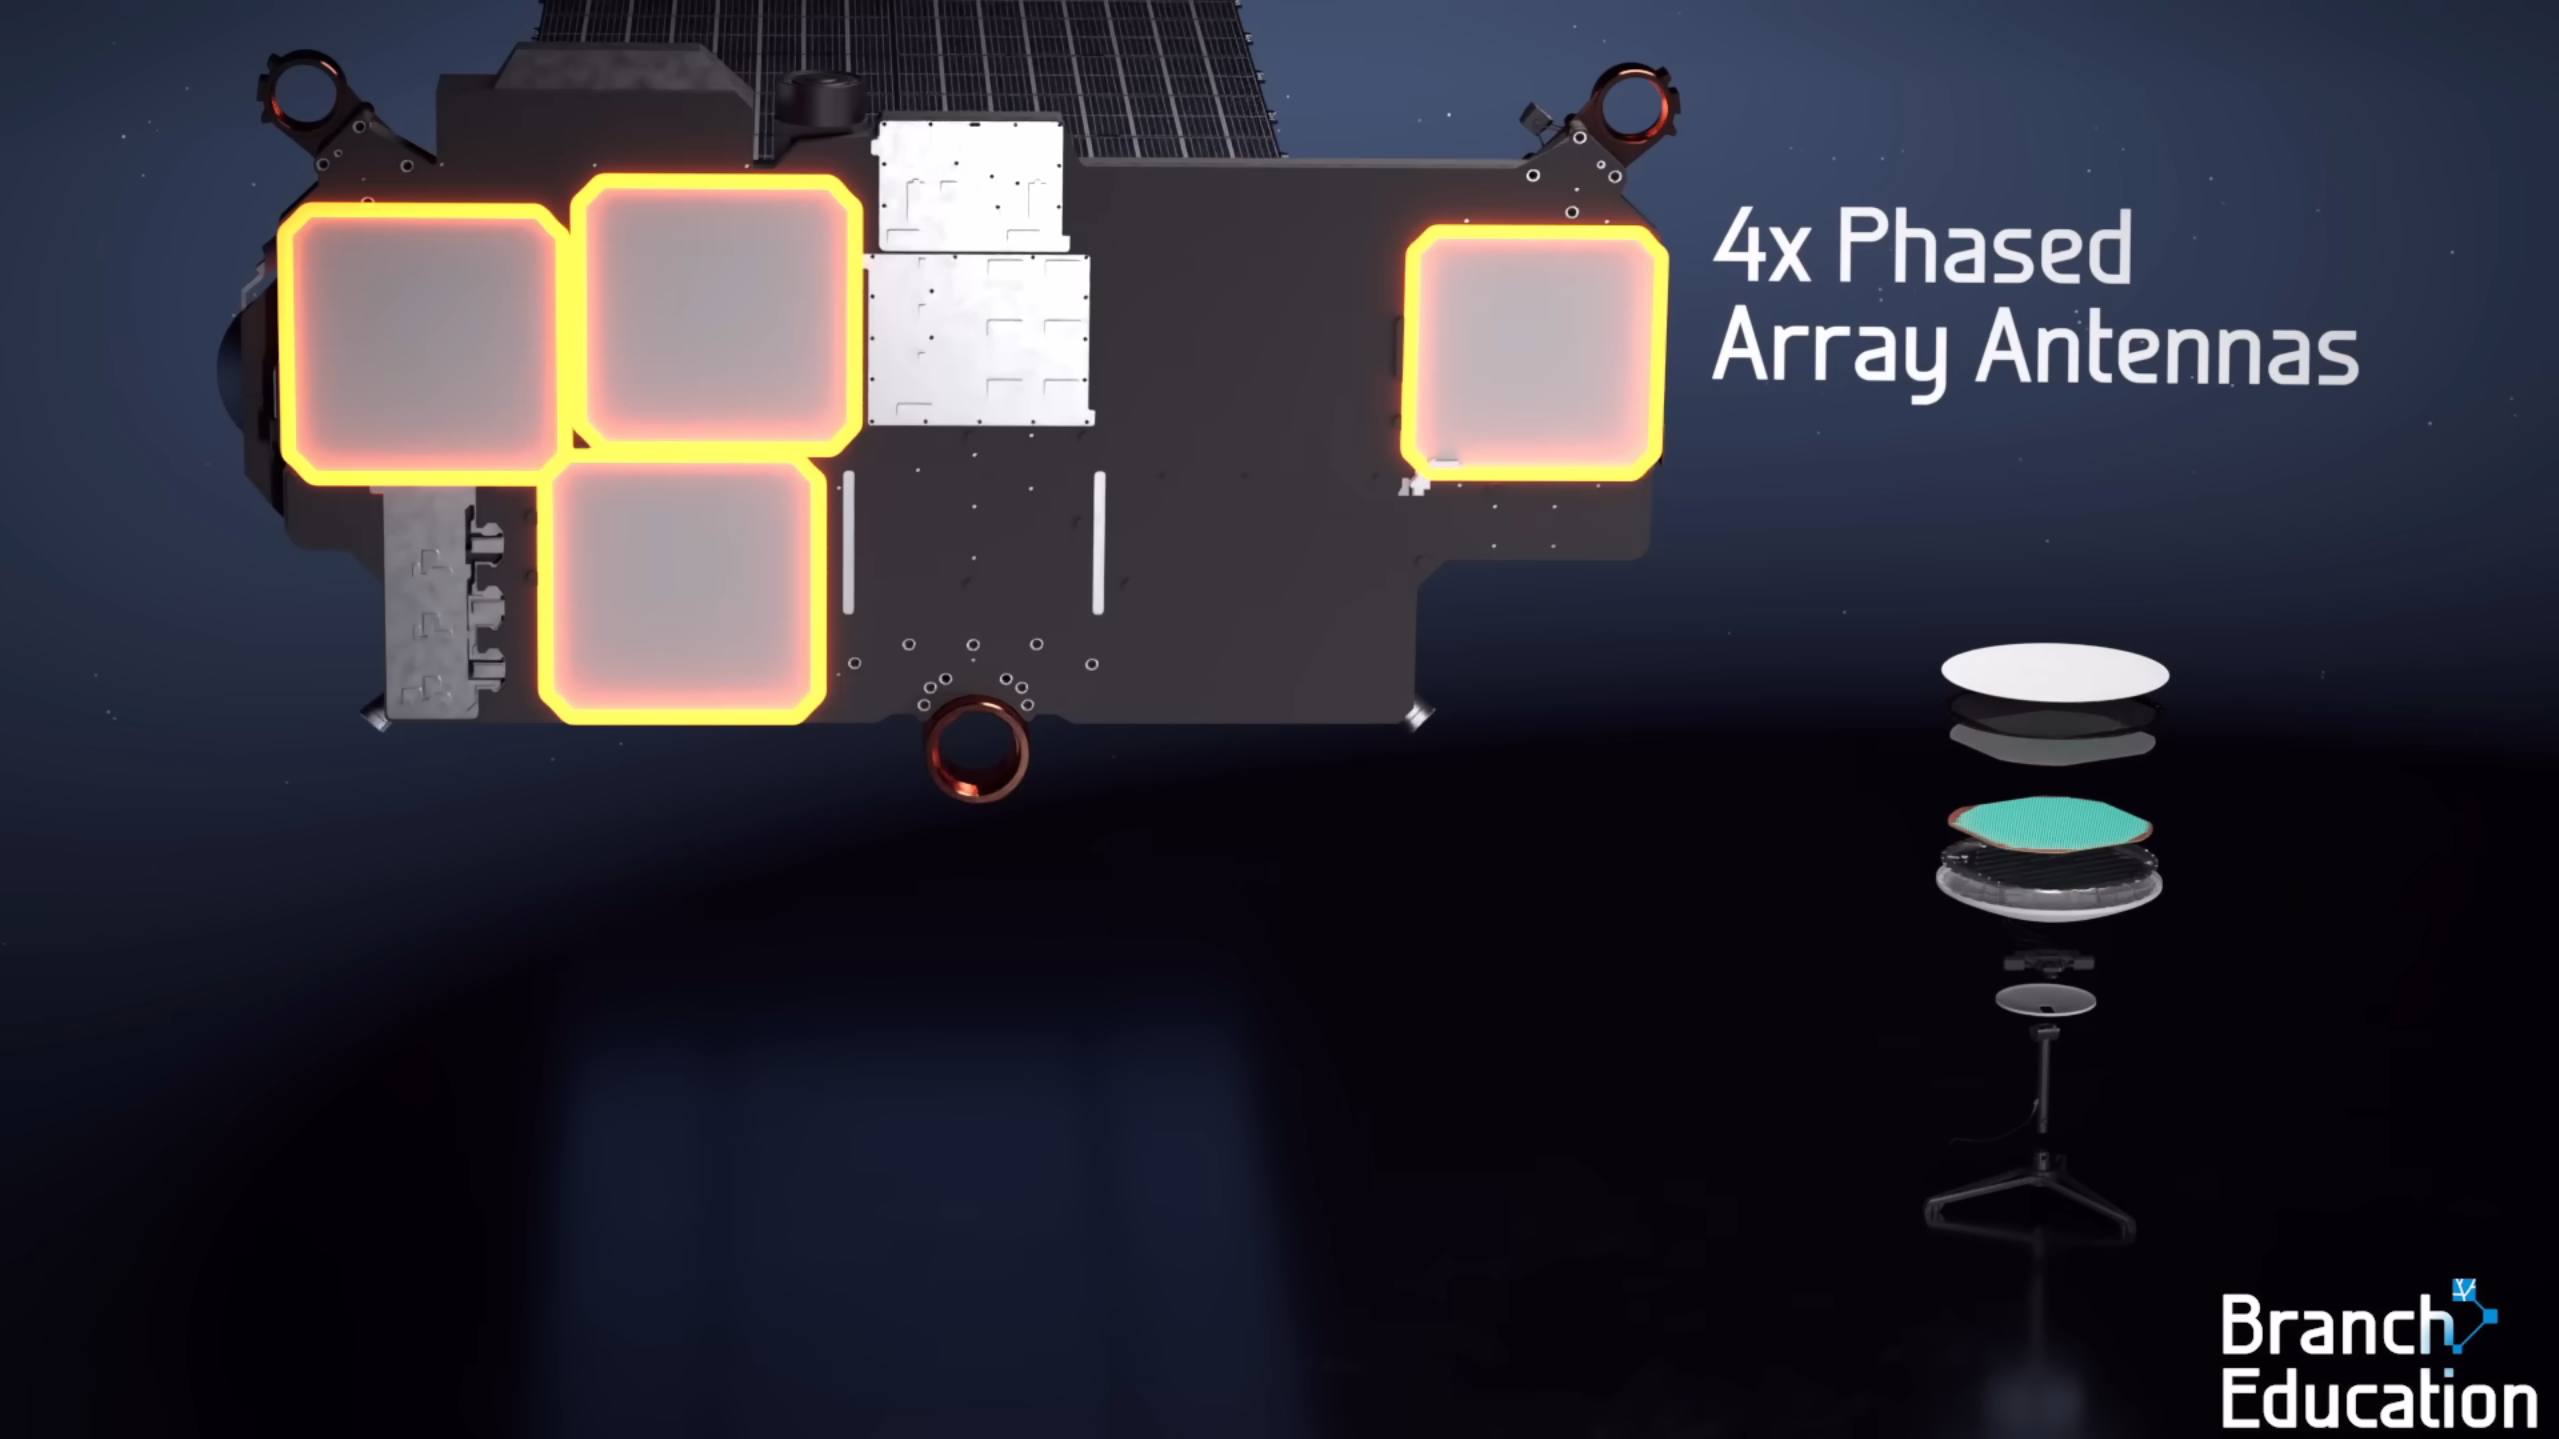
\includegraphics[width=\textwidth]{LaTeX/Figures/satellite_antennas.png}
        \caption{Satellite's antennas and dish. From~\cite{branch_education_starlink_2022}.}
        \label{fig:satellite_antennas}
    \end{subfigure}
    
\end{figure}

\begin{table}[h]
    \centering
    \caption{Key parameters for the selected satellite \textit{Starlink-3988} (NORAD ID 52625) as of October 2025. Data sourced from N2YO~\cite{n2yo_starlink3988}, In-The-Sky~\cite{inthesky_starlink3988}, StarlinkMap~\cite{starlinkmap.org}, and SpaceX public technical documentation~\cite{spacex_starlink_specs}.}
    \label{tab:starlink3988_params}
    \begin{tabular}{|l|c|c|}
        \hline
        \textbf{Parameter} & \textbf{Symbol / Unit} & \textbf{Value} \\ \hline
        NORAD Catalog Number & -- & 52625 \\ \hline
        COSPAR ID & -- & 2022-052AD \\ \hline
        Launch Date & -- & May 14, 2022 \\ \hline
        Launch Vehicle / Site & -- & Falcon 9 / Cape Canaveral (AFETR) \\ \hline
        Orbit Type & -- & Low Earth Orbit (LEO) \\ \hline
        Operational Status & -- & Active \\ \hline
        Starlink Model & -- & v1.5 (Laser Inter-satellite Links) \\ \hline
        Dimensions & -- & \SI{2.8}{\metre} $\times$ \SI{1.4}{\metre} $\times$ \SI{0.2}{\metre} (without solar array) \\ \hline
        Mass & $m$ (\si{\kilo\gram}) & 295 \\ \hline
        Inclination & $i$ (\si{\degree}) & 53.2 \\ \hline
        Semi-Major Axis & $a$ (\si{\kilo\metre}) & 6917 \\ \hline
        Perigee Altitude & $r_p$ (\si{\kilo\metre}) & 545.9 \\ \hline
        Apogee Altitude & $r_a$ (\si{\kilo\metre}) & 547.9 \\ \hline
        Mean Altitude & $h$ (\si{\kilo\metre}) & 546.9 \\ \hline
        Eccentricity & $e$ & 0.00014 \\ \hline
        Orbital Period & $T$ (\si{\minute}) & 95.4 \\ \hline
        Mean Motion & $n$ (\si{rev/day}) & 15.09 \\ \hline
    \end{tabular}
\end{table}


\newpage
\section{Data Collection}

To estimate the satellite's orbital period, two different methods were employed:

\begin{enumerate}
    \item Two overhead passes were tracked, with periodic logging of Azimuth and Elevation Angle parameters. In particular, the time of first appearance of the satellite above the horizon, followed by timestamps at every integer minute elapsed, and finally the time of disappearance of the satellite below the horizon, were all recorded. These values were then converted to Right Ascension and Declination, and, using these parameters from two distinct timestamps, the orbital period was estimated. (This corresponds to Method 1 in the instructions provided by the preceptors)
    \item The time at positions of constant elevation angle was recorded, and the orbital period was estimated as an average of these measurements. (This corresponds to Method 4 in the instructions provided by the preceptors)
\end{enumerate}

The results from the two methods were then compared and one of the two results was selected for the remainder of the calculations.

\subsection{Method 1}

The observations of \textit{Starlink-3988} for Method 1 were performed over two separate passes above the Princeton University Art Museum, New Jersey, United States, on 19 October 2025, using a combination of qualitative and quantitative tracking techniques. The \textit{Satellite Tracker} Android application (Vito Technology) was employed for qualitative tracking of the satellite in the night sky. We first used the app to obtain a prediction of the time of appearance of the satellite above the horizon. Then, the app was used to record both the time of appearance and disappearance of the satellite above and below the horizon. On the same Android phone, time was tracked to record the precise moment each integer minute would elapse. Concurrently, the \textit{Satellite Tracker Pro} iOS application (Kornienko Vyacheslav) was used on a separate Apple phone for quantitative measurements. In coordination with time tracking from the Android phone, we logged values of Azimuth and Elevation Angles, as well as the Distance from the observer to the satellite, through consecutive screenshots. By avoiding hand logging the data in real time, the three measurements were simultaneous, and, thus, any potential transient deviation was eliminated. The operation required two mobile phones and two people (the second person involved was my roomate, Tomás Consonni, an Economics student who kindly provided access to his iPhone). All times were logged in Eastern Daylight Time (EDT).

The observed Azimuth and Elevation Angles, measured from the Earth's surface, were converted to Right Ascension ($\alpha$) and Declination ($\delta$). This transformation to the equatorial coordinate system, which is relative to the Earth's barycenter, was performed using a Python script provided by the course preceptors. We input the coordinates of our observation station as \SI{40.3463}{\degree}N, \SI{-74.6580}{\degree}E, GMT-04:00. This code also uses the distance to the satellite as an additional input. The raw data are presented in Table~\ref{tab:method1_data} below. Screenshots of the two apps for the very last measurement on the second observation (10/20 at 19:38:16) are displayed in Appendix~\ref{Appendix}.

\begin{table}[H]
    \centering
    \caption{Raw empirical data for Method 1 observations}
    \label{tab:method1_data}
    \renewcommand{\arraystretch}{1.2}
    \begin{tabular}{|c|c|c|c|c|c|c|}
        \hline
        \textbf{Date} & \textbf{Time} & \textbf{Azimuth} & \textbf{Elevation} & \textbf{Distance} & \textbf{Right} & \textbf{Declination} \\ 
        \textbf{(2025)} & \textbf{(EDT)} & \textbf{(°)} & \textbf{Angle (°)} & \textbf{(km)} & \textbf{Ascension (°)} & \textbf{(°)} \\ \hline
        \multicolumn{7}{|c|}{\textbf{Observation 1 – 19 October 2025}} \\ \hline
        10/19 & 21:18:49 & 287.6 & 10.2 & 1628 & 315.8 & 42.8 \\ \hline
        10/19 & 21:19:00 & 286.3 & 11.0 & 1576 & 316.5 & 42.5 \\ \hline
        10/19 & 21:20:00 & 273.1 & 17.9 & 1226 & 321.0 & 39.9 \\ \hline
        10/19 & 21:21:00 & 262.7 & 21.8 & 1083 & 323.4 & 38.5 \\ \hline
        10/19 & 21:22:00 & 241.0 & 26.3 &  954 & 326.5 & 36.3 \\ \hline
        10/19 & 21:23:00 & 213.6 & 25.9 &  541 & 331.7 & 36.5 \\ \hline
        10/19 & 21:24:00 & 190.3 & 20.2 & 1137 & 333.0 & 31.2 \\ \hline
        10/19 & 21:25:00 & 176.0 & 13.7 & 1419 & 336.0 & 28.5 \\ \hline
        10/19 & 21:25:38 & 169.3 & 10.1 & 1657 & 338.0 & 26.5 \\ \hline
        \multicolumn{7}{|c|}{\textbf{Observation 2 – 20 October 2025}} \\ \hline
        10/20 & 19:31:03 & 319.7 & 10.5 & 1636 & 294.0 & 49.7 \\ \hline
        10/20 & 19:32:00 & 325.7 & 17.5 & 1264 & 299.3 & 48.2 \\ \hline
        10/20 & 19:33:00 & 337.5 & 28.0 &  930 & 304.2 & 46.4 \\ \hline
        10/20 & 19:34:00 & 006.1 & 42.2 &  694 & 308.9 & 44.4 \\ \hline
        10/20 & 19:35:00 & 056.7 & 43.7 &  677 & 313.2 & 42.2 \\ \hline
        10/20 & 19:36:00 & 088.6 & 29.9 &  886 & 317.2 & 39.9 \\ \hline
        10/20 & 19:37:00 & 101.9 & 18.6 & 1216 & 321.0 & 37.4 \\ \hline
        10/20 & 19:38:00 & 108.3 & 11.3 & 1579 & 324.4 & 34.9 \\ \hline
        10/20 & 19:38:16 & 109.5 & 09.8 & 1675 & 325.3 & 34.3 \\ \hline
    \end{tabular}
\end{table}

In preparation for the real observation, a test logging of data was also performed using the \textit{In The Sky} website. These data can be found in Appendix~\ref{Appendix} and do not contain distance to satellite entries.

\subsection{Method 4}

For the implementation of Method 4, we employed a similar experimental setup. Observations were conducted from Princeton University Art Museum, New Jersey, United States, during 21 October 2025. The \textit{Satellite Tracker Pro} iOS application (Kornienko Vyacheslav) was once again employed for quantitative tracking, while the iPhone’s built-in screen recording feature was activated overnight to capture the full sequence of satellite passes automatically. The recorded footage was later analysed to extract precise timestamps at which the satellite crossed a constant elevation angle during each pass. By repeating this process several times, a consistent dataset was obtained without the need for manual data entry, thereby reducing human timing errors. All times were recorded in Eastern Daylight Time (EDT), and each entry includes the corresponding distance from the observer to the satellite as provided by the application (to give an idea of which side of the earth the satellite was on). The elapsed times between consecutive passes at the same elevation will be used to estimate the orbital period. The raw data are to be entered in Table~\ref{tab:method4_data} below.

\begin{table}[H]
    \centering
    \caption{Raw empirical data for Method 4 observations}
    \label{tab:method4_data}
    \renewcommand{\arraystretch}{1.2}
    \begin{tabular}{|c|c|c|c|c|}
        \hline
        \textbf{Date (2025)} & \textbf{Time (EDT)} & \textbf{Elevation Angle (°)} & \textbf{Latitude (°N)} & \textbf{Longitude (°E)} \\ \hline
        \multicolumn{5}{|c|}{\textbf{Observations – 21 October 2025}} \\ \hline
        10/21 & 15:10:29 & -80.0 & -43.63 & 79.67\\ \hline
        10/21 & 16:49:20 & -80.0 & -58.24 & 72.31\\ \hline
        10/21 & & & & \\ \hline
        10/21 & & & & \\ \hline
        10/21 & & & & \\ \hline
        10/21 & & & & \\ \hline
        10/21 & & & & \\ \hline
        10/21 & & & & \\ \hline
        10/21 & & & & \\ \hline
        10/21 & & & & \\ \hline
    \end{tabular}
\end{table}





\section{Estimate of Period and Angular Velocity}

\section{Estimate of Semi-Major Axis and Position Prediction}

\section{Estimate of Orbital Elements}

\section{Error Analysis}

\section{Conclusion}

\section{Visualisation}

\printbibliography

\newpage
\appendix
\section{Appendix} \label{Appendix}

Screenshots of the mobile apps used for the observations. The screenshots show the last observation taken on 10/20, and are labelled to distinguish them from other similar screenshots. Figure~\ref{fig:tracker_screenshot} shows the Satellite Tracker mobile app in use on a Samsung Galaxy S24 Ultra. Figure~\ref{fig:tracker_pro_screenshot} shows the Satellite Tracker Pro app in use on an iPhone 12.

\begin{figure}[h!]
    \centering

    \begin{subfigure}[b]{0.4\textwidth}
        \centering
        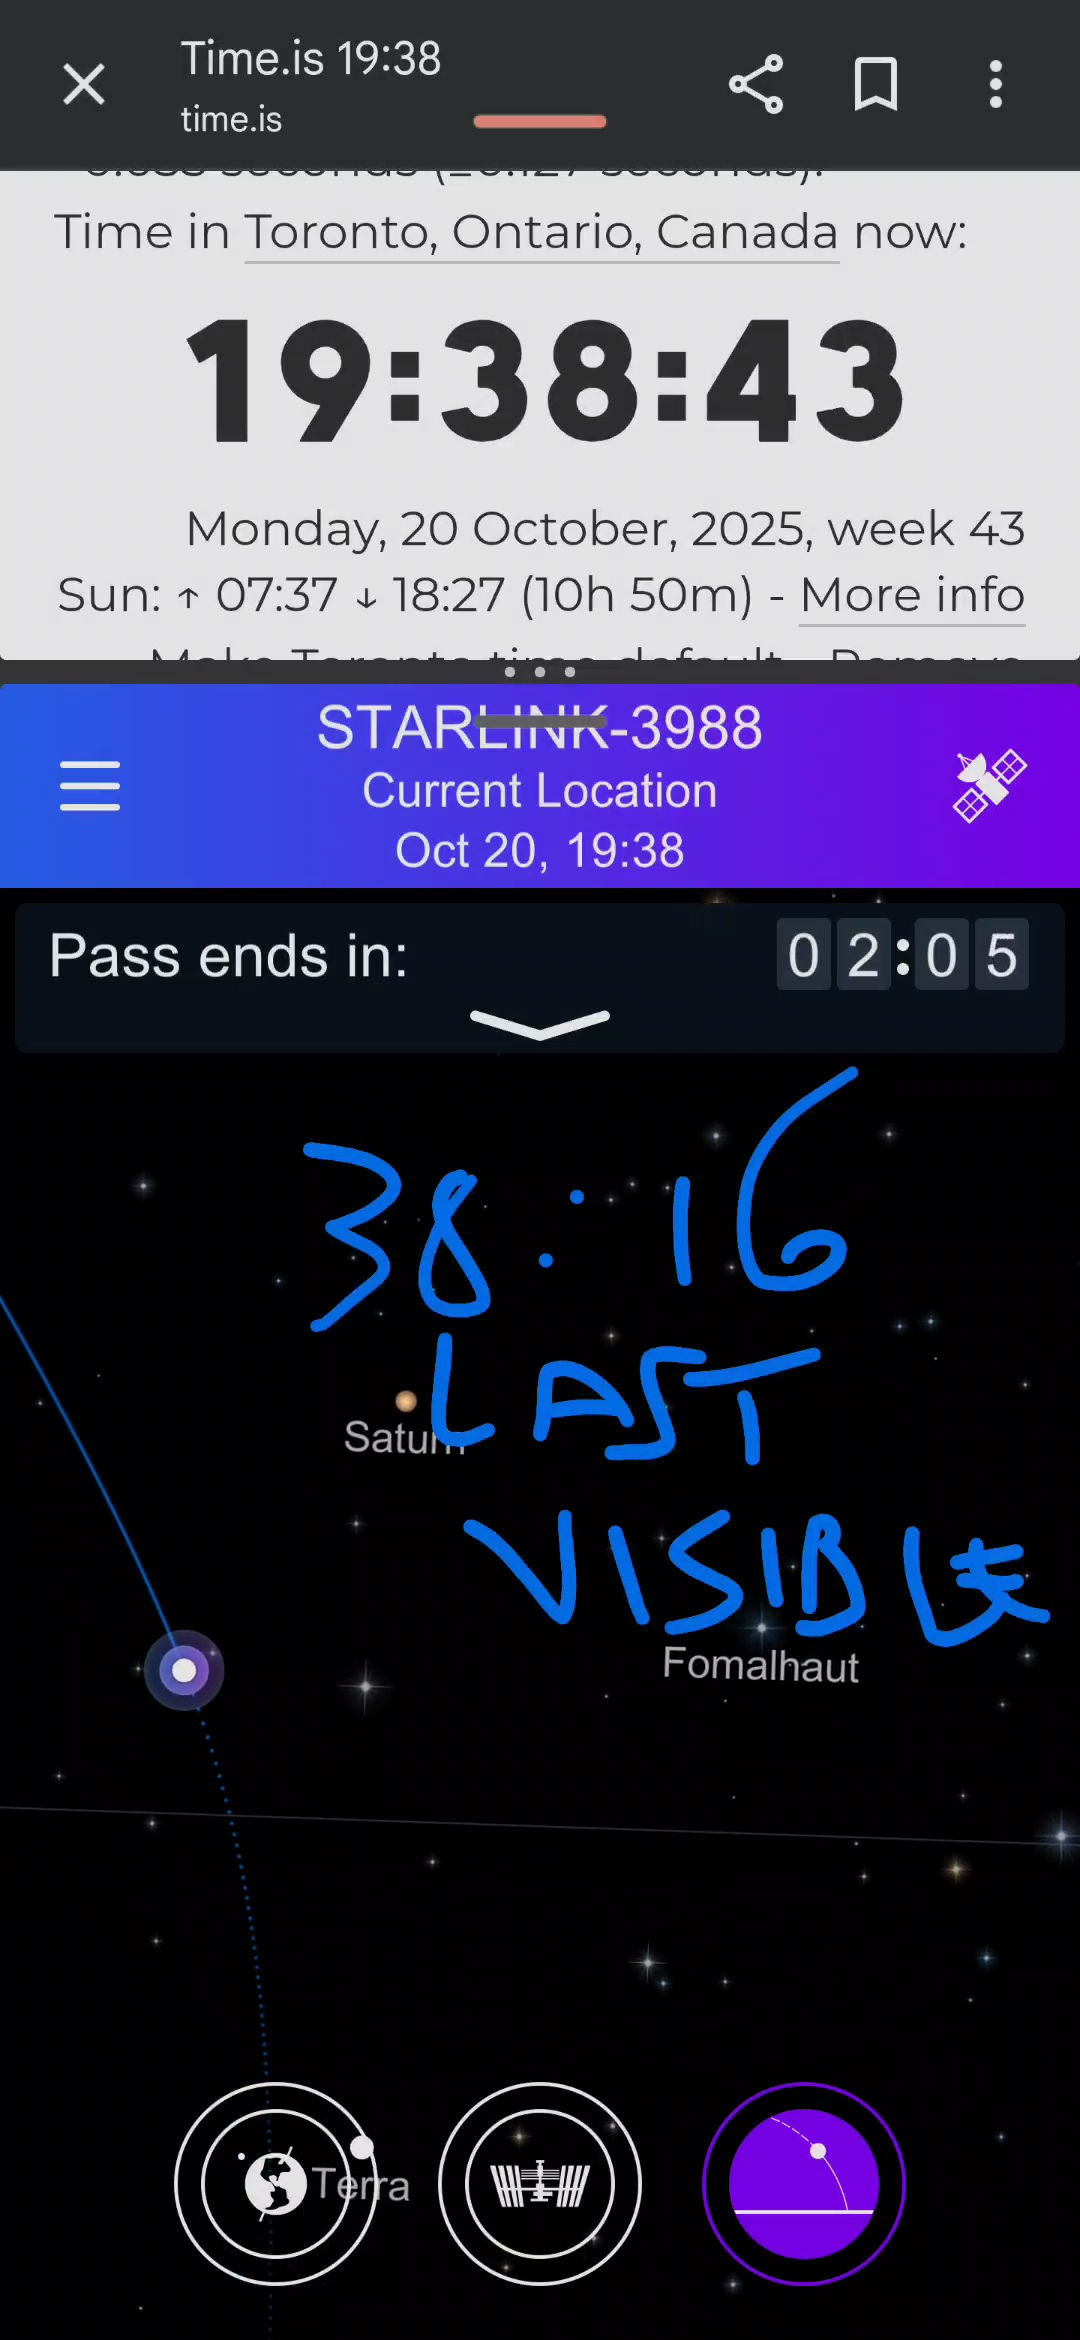
\includegraphics[width=\textwidth]{LaTeX/Figures/Satellite_Tracker_Screenshot.jpg}
        \caption{Satellite Tracker app}
        \label{fig:tracker_screenshot}
    \end{subfigure}
    \begin{subfigure}[b]{0.4\textwidth}
        \centering
        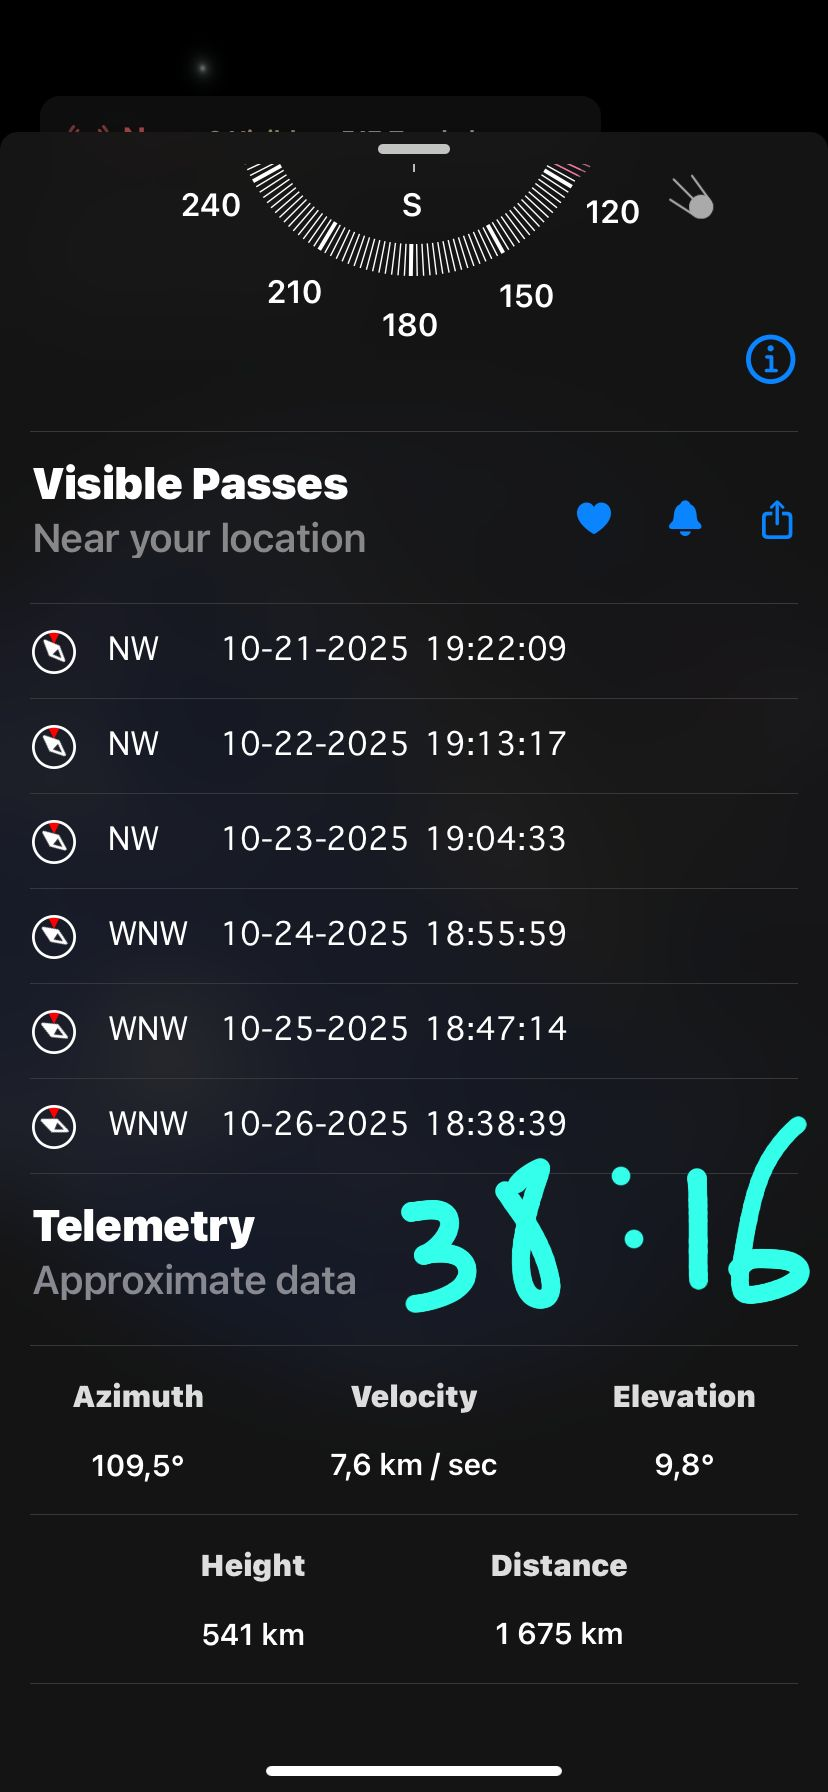
\includegraphics[width=\textwidth]{LaTeX/Figures/Satellite_Tracker_Pro_Screenshot.jpg}
        \caption{Satellite Tracker Pro app}
        \label{fig:tracker_pro_screenshot}
    \end{subfigure}
    
\end{figure}

\begin{table}[H]
    \centering
    \caption{Comparison data from the In The Sky website}
    \label{tab:method1_data_comparison}
    \renewcommand{\arraystretch}{1.2}
    \begin{tabular}{|c|c|c|c|c|c|}
        \hline
        \textbf{Date} & \textbf{Time} & \textbf{Azimuth} & \textbf{Elevation} & \textbf{Right} & \textbf{Declination} \\ 
        \textbf{ } & \textbf{ } & \textbf{(°)} & \textbf{Angle (°)} & \textbf{Ascension (°)} & \textbf{(°)} \\ \hline
        \multicolumn{6}{|c|}{\textbf{Observation 1}} \\ \hline
        10/19 & 19:39:15 & 321.0 & 10.0 & 189.3 & 43.8 \\ \hline
        10/19 & 19:40:00 & 324.5 & 13.9 & 189.5 & 49.3 \\ \hline
        10/19 & 19:41:00 & 333.4 & 21.7 & 188.3 & 60.8 \\ \hline
        10/19 & 19:42:00 & 350.5 & 32.1 & 175.8 & 78.7 \\ \hline
        10/19 & 19:43:00 & 024.8 & 41.0 & 029.8 & 71.3 \\ \hline
        10/19 & 19:44:00 & 061.3 & 37.0 & 023.0 & 43.0 \\ \hline
        10/19 & 19:45:00 & 084.6 & 26.1 & 022.3 & 20.4 \\ \hline
        10/19 & 19:46:00 & 096.2 & 16.9 & 022.8 & 06.3 \\ \hline
        10/19 & 19:46:29 & 102.5 & 10.2 & 023.8 & -03.7 \\ \hline
    \end{tabular}
\end{table}


\end{document}
